\documentclass[10pt,twocolumn,letterpaper]{article}

\usepackage{iccv}
\usepackage{times}
\usepackage{epsfig}
\usepackage{graphicx}
\usepackage{amsmath}
\usepackage{amssymb}
\usepackage{listings}
\usepackage{verbatim}
\usepackage{algorithm2e}
\usepackage{cite}

\long\def\sw#1{\textcolor{red}{**[SW] #1**}}
\long\def\ge#1{\textcolor{green}{**[GE] #1**}}
\long\def\dv#1{\textcolor{blue}{**[DV] #1**}}

\newcommand{\obs}{\mathbf{O}}
\newcommand{\state}{\mathbf{X}}
\renewcommand{\vec}[1]{\ensuremath{\overrightarrow{#1}}}


% Include other packages here, before hyperref.

% If you comment hyperref and then uncomment it, you should delete
% egpaper.aux before re-running latex.  (Or just hit 'q' on the first latex
% run, let it finish, and you should be clear).
\usepackage[pagebackref=true,breaklinks=true,letterpaper=true,colorlinks,bookmarks=false]{hyperref}

 %\iccvfinalcopy % *** Uncomment this line for the final submission

\def\iccvPaperID{****} % *** Enter the ICCV Paper ID here
\def\httilde{\mbox{\tt\raisebox{-.5ex}{\symbol{126}}}}

% Pages are numbered in submission mode, and unnumbered in camera-ready
\ificcvfinal\pagestyle{empty}\fi
\begin{document}

%%%%%%%%% TITLE
\title{Hard real time multi person detection}

\author{Deepak Geetha Viswanathan\\
University of Amsterdam\\
Science Park 904, Amsterdam\\
{\tt\small D.GeethaViswanathan@uva.nl}
% For a paper whose authors are all at the same institution,
% omit the following lines up until the closing ``}''.
% Additional authors and addresses can be added with ``\and'',
% just like the second author.
% To save space, use either the email address or home page, not both
\and
Gwenn Engelbienne\\
University of Amsterdam\\
Amsterdam\\
{\tt\small g.englebienne@uva.nl}
\and
Shimon Whiteson\\
University of Amsterdam\\
Amsterdam\\
{\tt\small s.a.whiteson@uva.nl}
\and
Ben Krose\\
University of Amsterdam\\
Amsterdam\\
{\tt\small b.j.a.krose@uva.nl}
}

\maketitle
%\thispagestyle{empty}


%%%%%%%%% ABSTRACT
\begin{abstract}
Trained object detectors are an important component of tracking by detection systems. For robust localization and tracking, computationally expensive detectors are needed, but are these are not usable in practice in an online setting.  In this work, we describe a novel multi person detection framework based on quantifying the uncertainty of camera observations at different world locations, and using it to prune the search space of a Dalal and Triggs detector. Online settings force us to adhere to hard computational constraints. We model our hard computational constraint as an action selection problem. By applying the principle of submodular functions, we have developed a greedy action selection scheme with theoretical gaurantees. This framework enables us to compute an accurate belief about the location of the people in the environment using a pruned set of input locations, thus reducing the computational load on the detection system and making accurate online tracking in challenging environments feasible in practice.
\end{abstract}

%%%%%%%%% BODY TEXT
\section{Introduction}
Multi-person detection is a key problem in computer vision.  In addition to its direct applications, in e.g., \sw{add examples with cites}, detection is also important as a subroutine in person tracking \sw{cite} frameworks.  

A key challenge in multi-person detection is to develop methods that work well in on-line settings in which hard computational constraints must be obeyed. For example, a mobile robot may require real-time  estimates of the location of people in its environment in order to perform socially aware navigation.  In such settings, high-quality detection often necessitates multiple cameras.  The volume of data generated by these cameras is then difficult to process within the given computational constraints.  

Existing state-of-the-art systems typically use either a \emph{detection by classification} framework~\cite{Pami-11} or detection by background subtraction method.

Detection by classification framework uses a trained shape based object detector. These detectors can model the overall shape of the person as well as individual body parts. The performance of these classification based detectors vary largely based on the granularity at which the shape of a human is abstracted.   
Detectors that exploit the overall shape of a person such as those based on a \emph{histogram of oriented gradients} (HOG)~\cite{dalaltriggs} are optimal to detect upright standing people. 
Nevertheless, in practical environments, it is difficult to filter out false positives caused by objects which appear to be human, like coat hangers, or social robots. By contrast, more sophisticated detectors model individual parts of the body using a \emph{deformable parts model} \cite{DPM} or a \emph{non-deformable mixture of parts model} ~\cite{partsDeva}. 
These parts-based detectors are typically more accurate for various poses than dalal and triggs detector. Trained object detectors are generally computationally expensive for an online setting. 

Methods based on an accurate model of the background, rather than a model of the foreground do not pose any computational constraints, but have some difficulties of their own. Background based methods can only detect people when they are in motion. This is a major difficulty in using them in indoor environments where people are involved in stationary activities. In a dynamic environments, the lighting conditions are very challenging. Moreover, while background-based methods are good at dealing with the large variety of poses and appearances of the foreground (people), they do not provide us with a principled way to interpret this foreground: it is very hard for the algorithm to work out which parts of the foreground are actually touching the ground, and therefore to map the observations in the image domain to the world domain.

In this paper, we present a new approach for multi-person detection that gets the best of both worlds.  In particular, it outperforms both the dalal and triggs as well as the background based detector, but with much lower computational costs than applying the dalal and triggs detector.  Furthermore, because it can obey hard computational constraints while making efficient use of whatever computational resources are available, it is ideally suited to on-line settings.

The main idea is to quantify the system's uncertainty about people's locations and use this to make smart choices about where to apply the expensive dalal and triggs detector.  In the off-line phase, we learn observation functions for each detector that estimate the probability of detection given people's true locations.  In the on-line phase, we apply the background based detector to all the images collected by the cameras and, using its observation function, compute a posterior distribution over people's locations.  Then, using this posterior and the observation function for the dalal and triggs detector, we select a subset of the windows in all the images that are estimated to maximize \emph{information gain}.  We then apply the dalal and triggs detector only to this subset and use the resulting detections to compute a second posterior, from which final predictions about people's locations can be made.  By making smart choices about where to apply the expensive dalal and triggs detector, this method can achieve high accuracy at much lower computational cost.  In adddition, since it works with window subsets of any size, it can easily be tuned to meet hard computational constraints.  

We evaluated our method on a real-world dataset gathered from a multi-camera system consisting of \sw{add details.}  Our results show that our method performs nearly as well as, but is much faster than, a standard dalal and triggs detector.  In addition, it substantially outperforms baselines that use only background based detectors or that naively combined both the detectors.

\section {Related work} \dv{To Edit}

%Motivate tracking by detection
Trained object detector is widely used for practical tracking scenarios~\cite{Pami-11}~\cite{POM-main}~\cite{MIL-obj1}. Background subtraction methods~\cite{bk1}~\cite{bk2-bayesian} are used far less in state of the art systems. Object detectors are more tolerant to illumination variations~\cite{ObjDet-1} and also can detect static people. Robust tracking systems can be built using  tracking by detection framework.

%Motivate Parts based models and their importance in tracking
Different techniques are available for detection with varying computational requirements. Until recently, overall shaped based models where used more predominantly as the object detectors, but in recent literature, the use of parts based models of the person is being explored~\cite{doubleperson}~\cite{Parts_tracking1}.
In ~\cite{Parts_tracking1}, they use the DPM model for tracking in difficult multi target scenarios. They exploit the potential of individual part detectors to reason about occlusions dynamically. In ~\cite{doubleperson} occlusions are handled using a specially trained detector to detect partially occluded pair of people. 
Altough these methods are applicable online, the computational cost of applying the parts detector is a concern. One of the requirements in using parts based models in tracking is the availability of high resolution data of the environment. Altough sensors which can provide such data is widely available, the applicability of parts based detectors in an online setting is a problem which is not addressed in any of the works. This is a shortcoming we have rectified in our work. 

%Motivate observation function
Another aspect of using the tracking by detection framework is to tranform the sliding window outputs to a useful likelihood function which can be used by a time dependent tracking framework. This is an important aspect of using trained detectors.  Conventional approaches of using a non maximal suppression and modelling the likelihood using suppressed detections throws away a large amount of information provided by the detector in an ad-hoc way. This reduces the efficiency of the bayesian tracker which then uses the non-maximally suppressed output. In ~\cite{POM-main} all the detections from different locations are used to build a probablistic likelihood map. The idea of using a more descriptive likelihood is used in several recent works. In ~\cite{Pami-11} the authors use the confidence values of the detector at different image locations for creating a likelihood function which they later use for particle filter based tracking. In our work, we emphasize the importance of a learnt observation model for transforming the detector results. Performance of standard detectors on a specific environment is highly variable depending on illumination conditions, density of crowd, height of camera placement, and many other factors which cannot be explicitly quantified. The most general way of being able to apply standard detectors on various environments is to quantify the performance of the detector using domain specific data by learning an observation model. Section 5 explains the generic observation model which can be learnt from labelled data.

%Motivate action selection
The problem of dynamic resource allocation has been widely researched in the area of sensor networks. We can classify the exisisting techinques into non-myopic and myopic planning techniques.  Decision theoretic framework of POMDP~\cite{Kaelbling98}, provides a theoretically sound backbone for incorporating non myopic control in bayesian systems. Dynamic planners using POMDP have been successfuly used in sensor selection scenarios~\cite{Spaan09}, where optimal selection of cameras using temporal planning (given a  fixed computational budget) can provide a performance benefit over greedy sensor selection. In more complex scenarios, where it is not tractable to solve the large state-action spaces using POMDP (temporal planning methods), more pragmatic yet principled methods such as subodularity based greedy action selection have also proved to provide gauranteed performance benefits. In ~\cite{krause2012near} they propose the idea of using information gain as an objective function for the subset selection problem. They also prove that information gain as objective function is submodular. Nevertheless, the idea of resource allocation in high level computer vision algorithms is still an under explored area.Specifically, what we are interested in is a budgeted use of the outputs of the sensors (or detectors), in a principled way so as to not losing on the tracking performance. We exploit the submodularity property of information gain for smart use of the computationally expensive parts based detector.


\section{Problem Setting}

%\subsection{Environment and Cameras}
An indoor environment is considered in our work. $ n$ People are assumed to move on the ground plane of this environment. The ground plane is discretised into cells. Each of the cells can occupy at most one person at a time. We want to track the people using $ k $ wide field of view, calibrated, omni directional cameras. The cameras are mounted on the ceiling facing the ground plane, with the camera axis perpendicular to the ground plane. Each camera $ c $ observes a subset of the total cells.  The location of all the people in the environment is the true state of the world. This is represented by  \textbf{X} which stands for the true occupancy of all the cells. \textbf{X} consists of state features $X_{i}$, which represents the true occupancy of one cell $ i$. Each $X_{i}$ can take a binary value depending on the occupancy. $|\textbf{X}| $ is the total number of cells. The quality of perception depends on the subset of the cells observed by the camera and also on the location of the people in the environment.

For any given cell, the projection of the shape of a person in the image can be approximated by a rectangular window. This rectangular window or the sub-image at cell $ i $ from camera $ c$ is represented by $ I^{c}_{i} $. The sub-images (windows) are extracted and evaluated by a detection algorithm (detector). An action represents the selection of one of these windows as input to the detector. The joint action (of selection multiple windows) is specified by a binary  vector of size $|\textbf{X}| $.

A detector is a discriminatively trained classifier which takes as input a window and outputs a binary decision on the presence or absence of a person in that window. We consider the use of two detectors, a background based model and the Dalal and Triggs detector.

The computational constraint allows us to process all the windows for the background based model, but it allows us only to process $ K $ windows of the dalal and triggs detector. This is the problem we are trying to solve. How to choose the best $K$ window locations to apply the dalal and triggs detector.

%The HOG detector is applied on all windows for all cameras since it is computationally affordable to use it in an online setting. %(or in other words the joint action vector has a binary value of 1 for all the elements). 
%This output $O^{c}_{i} $ is used to compute the belief about the location of the  $ n $ people. This is a coarse estimate of the location of the people and is inaccurate. For a more accurate estimate of the belief we need to use the output of the parts based detector.

%It is practically impossible to apply the parts based detector on all the windows online. We need to select a subset of the windows while minimizing the loss of information. A principled way to choose the most informative set of windows is to model the uncertainity in the observation vector $ \textbf{O}$ (classifier output for all the windows) conditioned on the true state $\textbf{X} $ (location of the people) of the world and to use this observation model to select the subset of windows (action selection) which minimize the uncertainity of the state. \\

%The  joint action decides which windows to select to apply the detection algorithm. %A perception agent has control over the joint action i.e the agent decides which of the windows to select as input to the classifier.\\

%Two problems - 1. the observation model has a high dimensionality. How to model it practically.
%2. How to perform this action selection in an 'optimal' way - use the concept of adaptive submodularity.


\subsection{List of symbols}
\begin{table}[ht]
  \begin{tabular}{lll}
   \hline
   Symbol & Explanation \\
   \hline
   $C $ & Number of cameras\\
   $\textbf{G} $ & Number of cells\\
   %$G_{c} $ & Set of all cells visible from camera $c$.\\
   $ \textbf{I}^{c} $ & Raw input image from camera $ c$\\
   $ I_{i}^{c} $ & Raw image at location (Window) $ i$\\
   %$ W_{i}^{c} $ & Window at location $ i$\\
   $ \textbf{O} $ & Observation map - Classifier output for all  $ i $, $ c $\\
   $O^{c}_{i} $& Detector output for groundplane location $ i $\\
   $\textbf{X}$& True state (occupied/not occupied) for all $i$\\
   \hline
  \end{tabular}
  \caption{%
    Symbols.
  }
  \label{tab:Formal symbols}
\end{table}

\section{Proposed active data fusion framework}

\subsection{System architecture}
We first begin with the schematic representation of the system. Refer to figure 1.

\begin{figure*}
\begin{center}
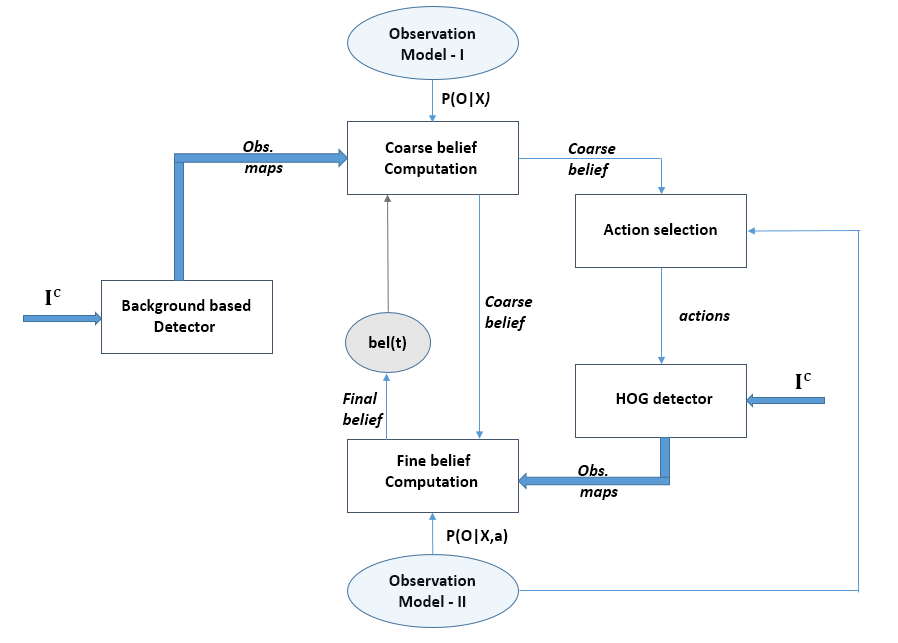
\includegraphics[width=12cm]{img/block_dia_cir.PNG}
\end{center}
   \caption{A schematic diagram of the proposed active data fusion system}
\label{fig:Block dia}
\end{figure*}

\subsection{Overview of the process}
As mentioned in the introduction, an iterative coarse to fine state estimation process is proposed in our work. This process utilizes two modules which are trained offline. 

\subsubsection{Offline learning}
\textbf{Module 1 - Background based detector}\\
A template based background model is used.\\
\textbf{Module 2 - Dalal and Triggs detector}\\
A standard 64*128 HOG based dalal and triggs detector is used in our system. Any detector which can be applied in an online setting can be used as an alternative. We have used the dalal and triggs detector since it is the most standard and widely used detector available.\\ 
\textbf{Module 3 - Observation model for background based detector}\\
Using ground truth labelled data and the background based detector output, an observation function is learnt for the background based detector\\
\textbf{Module 4 - Observation model for dalal and triggs detector}\\ 
Similar to module 3, an observation model is learnt offline for each camera which relates the output of the classifer to the true location of the people in the environment (true state). More details are discussed in section 5\\

\subsubsection{Online sequential process}
At time $t $, an image is acquired from all cameras synchronously. The detector output from the HOG detector is used to create an observation map.\\
\textbf{Step 1 - Coarse state estimation}\\
The next step is estimating the state of the world using sampling. Using the detector output map and the learnt observation function for the HOG detector, we compute the MAP estimates of the location of the people in the world (state) using MCMC sampling.\\ 
\textbf{Step 2 - Action section}\\
In the next step, the greedy action selection mechanism (agent) will
decide the window locations (from each camera) to be selected for applying the parts based detector, using the coarse belief and the observation function for the parts based detector.\\
\textbf{Step 3 - Fine state estimation}\\
Based on these actions (i.e. extracted new features)
and the learnt observation model incorporating these features, fine state estimation is performed to obtain the final corrected state estimates.

The different modules invovled in the system is explained in detail in the following sections.

\section{Observation function}
The detectors, the performance of the classifier for different world states needs
to be quantified. We need to learn an observation function which willcorrelate the output of the classifier $O^{c}_{i}$ to different world
states $X_{j}$.
This observation function will tell us the probability of
obtaining the observation $ O^{c}_{i} $, from the detector that a grid cell is occupied (or not occupied) given the true location of all the people in the environment(the true state of the world ($ X_{j},\forall j $).We need to learn $ P(\textbf{O}|\textbf{X})  $\\

The two observation functions for the HOG detector and the parts based detector is explained below:

\subsection{Factorization}

The observation function will have very high dimensionality if represented in the naive form. It would be beneficial to simplify this observation function.

We can consider that the observations from each grid cell are independent of one another conditioned on the true state.
\begin{align}
P(\textbf{O}|\textbf{X})&=\prod_{c,i} {P(O_{i}^{c}|\textbf{X})}
\end{align}

Next we could reduce the dimensionality of state space if we consider only a neighbourhood around $ X_{i} $, instead of the whole occupancy $\textbf{X} $. The output of a window at location $ i $ is only affected by its own occupancy and a neighbourhood of windows which overlaps with the window at $ i$. This approximation can be represented as follows:\\ 

\begin{align}
  P(\obs|\state) &= \prod_{c,i} \, P(O_{i}^{c}|X_{i},X_{n_{c}(i)})
\end{align}

We now need to compute  $ P(O_{i}^{c}|X_{i},X_{n_{c(i)}}) $. Depending on the values that $ X_{i} $, $ X_{n_{c(i)}} $ can take we have six distinct scenarios of occupancy. In the next subsection we will explain how to model the observation function in terms of image features for these scenarios.    \\

\subsection{Representation of observation function parameters}

Based on the neighbourhood occupancy, we can have three distinct cases : empty neighbourhood, single person in the nieghbourhood and multiple people in the neighbourhood. In each of these cases we need to learn a likelihood function over different image parameters which captures the essential state features such as occlusion, distance from camera, occupancy of the cell and its neighbours. The image features (pseudo distances) based method enables us to generalize the important aspects of the state space which affects the detector performance. This helps us to learn an observation function over these pseudo distance parameters from a tractable amount of labelled data.\\

\textbf{Empty neighbourhood}

\begin{align}
 P(O^{c}_{i} |X_{i}=\alpha ,\forall j \in{n_{c(i)}},X_{j} =0)  &=\mu^{0}_{\alpha}
\end{align}

The functions $ \mu^{0}_{0} $  and $ \mu^{0}_{1} $ is learnt from training data. \\

\textbf{One person in the neighbourhood}\\
Let us consider that one of the neighbours of $ i$ is occupied. This occupancy affects the classifier response at $ i$. We need to consdier two cases seperately. The scenario in which $ i $ is occupied and the alternative, in which $ i$ is empty.

In order to quantify the effect of neighbourhood occupancy, we need to consider a pseudo distance between $I_{i}^{c}$ and $I_{j}^{c}$.
 
In order to quantify the effect of neighbourhood occupancy, we need to define a pseudo distance function between $I_{i}^{c}$ and $I_{j}^{c}$.

\begin{align}
\alpha(i,j) = \sqrt{\Vert I_{i}^{c}\Vert/\Vert I_{j}^{c}\Vert}
\end{align}

\begin{align}
\beta(i,j) = \delta^{c} (i,j)\times \sqrt{\Vert I_{j}^{c}\Vert}
\end{align}
 
 where $\delta^{c} (i,j)$ is the distance between the centres of $I_{i}^{c}$ and $I_{j}^{c}$.
 
\begin{align}
 P(O^{c}_{i} |X_{i}=0 , j \in{n_{c(i)}},X_{j} =1)  &=\mu^{1}_{0}(     \alpha(i,j),\beta(i,j))
\end{align}



For the case when $ i $ is occupied, we need to encode the fact that the neighbourhood in front of $i$ w.r.t to the camera is different from the neighbourhood behind $ i$ w.r.t the camera. Similar to the first case we need to define a pseudo distance function, which is given by :
\begin{align}
\gamma(i,j) = \Vert I_{i}^{c}\cap I_{j}^{c} \Vert / \Vert I_{i}^{c}\Vert \times (1 - \Vert I_{i}^{c}\cap I_{j}^{c} \Vert /\Vert I_{j}^{c}\Vert) 
\end{align}

\begin{align}
\begin{split}
P(O^{c}_{i} |X_{i}=1 , \exists j \in{n_{c}(i)}: X_{j} =1,\\ \forall k \neq j, X_{k} =0)  &=\mu^{1}_{1}(  \gamma(i,j))
\end{split}
\end{align}

 Using these pseudo distances we can generalize the observation model for any single occupancy configuration.\\

\textbf{Multiple people in the neighbourhood}\\
Let us define 
\begin{align}
 \textbf{J}_{i}^{c} = argmax_{j\in n_{c(i)},X_{j}=1} \Vert I_{i}^{c}\cap I_{j}^{c} \Vert  
\end{align}

\begin{align}
 P(O^{c}_{i} |X_{i}=0 ,\exists j  \in{n_{c(i)}},X_{j} =1)  &=\mu^{2}_{0}(     \alpha(i,j),\beta(i,j))
\end{align}

\begin{align}
 P(O^{c}_{i} |X_{i}=1 ,\exists j \in{n_{c(i)}},X_{j} =1)  &=\mu^{2}_{0}(  \gamma(i,j))
\end{align}


\section{Belief computation}

\section{Action Selection}

\subsection{List of symbols}
\begin{table}[ht]
  \begin{tabular}{lll}
   \hline
   Symbol & Explanation \\
   \hline
$\textbf{X} $ & State of the world\\
 $\mathcal{X} $ & Set of samples of $\textbf{X}$ \\
 $\textbf{W} $ & Set of all possible actions\\
 $K$ & Maximum number of actions in one time step\\
 $\mathcal{A} $ & Set of selected actions\\
 $\mathcal{A}^{k} $ & Set of selected actions at intra time step $k$\\
 $\underline{\mathcal{A}} $ & Detector results corresponding to $\mathcal{A}$\\
 $a $ & An action\\
 $ \underline{a} $ & Detector results corresponding to $ a$\\
   \hline
  \end{tabular}
  \caption{
    Symbols - action selection
  }
  \label{tab:Symbols in action selection}
\end{table}

The Dalal and Triggs detector is to be applied on a pruned set of windows. A unit action corresponds to selecting a window for applying the dalal and triggs detector. Joint action is the set of windows selected at every time step. 

We need to incrementally build a set of actions of size $ K $, where $ K $ represents our computational budget for applying the dalal triggs detector at every time step. 

One way to solve this problem is to use greedy maximization with respect to a metric such as information gain for each of the possible actions. So we want to use information gain to quantify the "value" of all possible actions and then incrementally build the set of actions greedily.
  
We use information gain as the objective function to pick the most informative action.
We need to compute $I^{k}(\textbf{X};a)$ and pick the $a$ which maximizes the information gain. More formally,

\begin{align}
a^{k} = \operatorname*{arg\,max}_{a\in W \setminus A} I^{k}(\textbf{X};a)
\end{align}

This selected action is added to $\mathcal{A}^{k}$\\
For the action selection task,
\begin{align}
\operatorname*{arg\,max}_{a\in W \setminus{\mathcal{A}}}I^{k}(\textbf{X}; a) =\operatorname*{arg\,max}_{a\in W \setminus{\mathcal{A}}} (H^{k}(\textbf{X}) - H^{k}(\textbf{X}|a))
\end{align}
\begin{align}
a^{k+1} =\operatorname*{arg\,max}_{a\in W \setminus{\mathcal{A}}} (- H^{k}(\textbf{X}|a))
\end{align}
In order to perform this action selection, we need to compute $H^{k}(\textbf{X}|a)$ for each $a$
\begin{align}
H^{k}(\textbf{X}| a) = -\sum_{\underline{a}\in\lbrace 0 ,1 \rbrace} \sum_{\textbf{X}} P^{k}(\underline{a})P^{k}(\textbf{X}| \underline{a}) \log(P^{k}(\textbf{X}| \underline{a}))
\end{align}
Applying bayes rule to the term inside log,

\begin{align}
H^{k}(\textbf{X}| a)= -\sum_{\underline{a}\in\lbrace 0 ,1 \rbrace} \sum_{\textbf{X}} P^{k}( \underline{a})P^{k}(\textbf{X}| \underline{a}) \log(\dfrac{P^{k}( \underline{a}|\textbf{X})P^{k}(\textbf{X})}{P^{k}( \underline{a})})
\end{align}

\begin{align}
\begin{split}
 = -\sum_{\underline{a}\in\lbrace 0 ,1 \rbrace} \sum_{\textbf{X}} P^{k}( \underline{a})  P^{k}(\textbf{X}| \underline{a}) \\ \Big\lbrace\log(P^{k}( \underline{a}|\textbf{X})P^{k}(\textbf{X})) - \log(P^{k}( \underline{a}))\Big\rbrace
\end{split}
\end{align}

There are two problems to be addressed
\begin{itemize}

\item{Equation (17), cannot be computed exactly since the possible values $\textbf{X}$ is large. We use sampling to approximately compute the value of equation 7.}

\item{Computing $P( \underline{a})$, which occurs several times in the previous equation needs to be done by marginalizing over $\textbf{X}$.Sampling is used for this computation as well.} 
\end{itemize}

\begin{align}
 P(\underline{a}) = \sum_{\textbf{X}}P( \underline{a}|\textbf{X})P(\textbf{X}))
\end{align}
%In order to obtain samples of \textbf{X} under the posterior $P^{k}(\textbf{X})$ at intra-time step $k$, we use an MCMC approch as described below.\\
\subsection{MCMC sampling}
At every intra time step, we need to use multiple MCMC sampling.
\begin{itemize}
\item Sample from the current posterior, $P^{k}(\textbf{X})$.

Use the detector output from the background based detection and the selected $k-1$ actions as the initial sample of the state $x^{'} $ and randomly flip a state feature $X_{i}$ to obtain a new proposal $x $.\\
Next step is to compute the acceptance probability and then accept or reject $x$.\\
The acceptance probability given by:
\begin{align}
A(x|x^{'}) = \min\Big\lbrace\Big(\dfrac{P(bk|x)P(\underline{\mathcal{A}}^{k}|x)}{P(bk|x^{'})P(\underline{\mathcal{A}}^{k}|x^{^{'}})}\Big),1\Big\rbrace
\end{align}

After the sampling we have a set of samples, represented by,
 $\mathcal{X}^{k}={\lbrace x^{k}_{i}\rbrace}^{N}_{i=1}$.\\
Let us substitute $\widehat{p}( \underline{a})$ for the quantity we estimate for $P( \underline{a})$ using the samples $\mathcal{X}^{k}$, in equation (18).
\begin{align}
\widehat{p}( \underline{a}) = \dfrac{1}{N}\sum_{x^{k}_{i}\in \mathcal{X}}P( \underline{a}|x_{i}^{k})
\end{align}


\item Sample from $P^{k}(\textbf{X}|\underline{a})$. (ficticious posterior)

Here we first select one of the remaining actions and together with the observed detector outputs at every time step as the initial sample of the state $x^{'} $ and randomly flip a state feature $X_{i}$ to obtain a new proposal $x $.\\
Next step is to compute the acceptance probability and then accept or reject $x$.\\
The acceptance probability given by:
\begin{align}
A(x|x^{'}) = \min\Big\lbrace\Big(\dfrac{P(bk|x)P(\underline{\mathcal{A}}^{k}\cup \underline{a}|x)}{P(bk|x^{'})P(\underline{\mathcal{A}}^{k}\cup \underline{a}|x^{^{'}})}\Big),1\Big\rbrace
\end{align}
\end{itemize}
After the sampling we have a set of samples, represented by,
 $\mathcal{X}^{k+1}={\lbrace x^{k+1}_{i}\rbrace}^{N}_{i=1}$.
\begin{align}
\begin{split}
H^{k}(\textbf{X}| a)\approx -\dfrac{1}{N}\sum_{\underline{a}\in\lbrace 0 ,1 \rbrace} \sum_{x_{i}^{k+1}\in\mathcal{X}^{k+1}} \widehat{p}( \underline{a})\\ \Big\lbrace\log(P( \underline{a}|x^{k+1}_{i})P(x^{k+1}_{i})) - \log(\widehat{p}( \underline{a}))\Big\rbrace
\end{split}
\end{align}

$P(x^{k+1}_{i})$ cannot be computed directly from the samples $\mathcal{X}^{k+1}$ alone. But we can compute this term using the samples from $\mathcal{X}^{k}$ and $\mathcal{X}^{k+1}$
\begin{align}
\begin{split}
H^{k}(\textbf{X}| a)\approx -\dfrac{1}{N}\sum_{\underline{a}\in\lbrace 0 ,1 \rbrace} \sum_{x_{i}^{k+1}\in\mathcal{X}^{k+1}} \widehat{p}( \underline{a}) \\ \Big\lbrace\log\Big(P( \underline{a}|x^{k}_{i})(\sum_{x_{j}^{k}\in\mathcal{X}^{k}}P(x^{k+1}_{i}|x^{k}_{j}))\Big) - \log(\widehat{p}( \underline{a}))\Big\rbrace
\end{split}
\end{align}
\textbf{Note} :
For each of the action to be evaluated at an intra-time step, we have three set of samples. One set of samples from the previous intra time step, and two sets of samples for the current intra time step, one set for $\underline{a}=1$ and another for $\underline{a}=0$ (fictious update).
  
\section{Experimentation}

\textbf{Data currently available}\\ 
Two sequences (single camera) multi person(three people). 1500 labelled windows in each data set. One sequence will be used for learning the observation function and tuning the detectors.The other sequence will be used for testing the performance of our system.\\

\textbf{Further data collection}\\
Collect multi camera dataset (two sequences).\\

\textbf{Systems to evaluate}\\
1. Dalal and Triggs\\ 
2. Naive Parts Based\\ 
3. Dalal and Triggs + Naive parts based (all windows) - \\
4. Dalal and Triggs + Naive parts based (Random windows)\\
5. Dalal and Triggs + Naive parts based (Sampling from prior)\\
6. Dalal and Triggs + Naive parts based (Pruned windows - proposed method)\\
 

\textbf{Evaluation procedure}\\
Tracking is evaluated using multi object detector accuracy and multi object detector precision.

\section{Discussion}


\section{Conclusion and Future work}
{\small
\bibliographystyle{ieee}
\bibliography{iccvbib}
}

\end{document}
